\begin{frame}[plain]
  \vfill
  \centering
  \Huge Multimodal Architectures
  \vfill
\end{frame}

\begin{frame}{Example: Trimodal Video Classification}
  \begin{columns}
    \begin{column}{0.55\textwidth}
      \textbf{Scoring how much each segment of a lecture video matters:}\\[0.4em]
      \begin{itemize}
        \item \textbf{Inputs:}
          \begin{itemize}
            \item \alert{Text} (subtitles) $\rightarrow$ textual encoder $\theta_T$
            \item \alert{Audio} (soundtrack) $\rightarrow$ audio encoder $\theta_A$
            \item \alert{Visual} (video frames) $\rightarrow$ visual encoder $\theta_V$
          \end{itemize}
        \item \textbf{Feature Extraction:}
          \begin{itemize}
            \item Each stream passes through its own BiLSTM layer ($64$ units)
          \end{itemize}
        \item \textbf{Fusion and Prediction:}
          \begin{itemize}
            \item The three feature vectors are concatenated
            \item Then a further BiLSTM ($64$) $\to$ Dense ($32$) $\to$ Dense ($16$) $\to$ output
            \item Final output: an importance score for the current segment
          \end{itemize}
        \item Each modality keeps its own encoder; they meet only at the concatenation.
      \end{itemize}
    \end{column}
    \begin{column}{0.43\textwidth}
      \begin{figure}
        \centering
        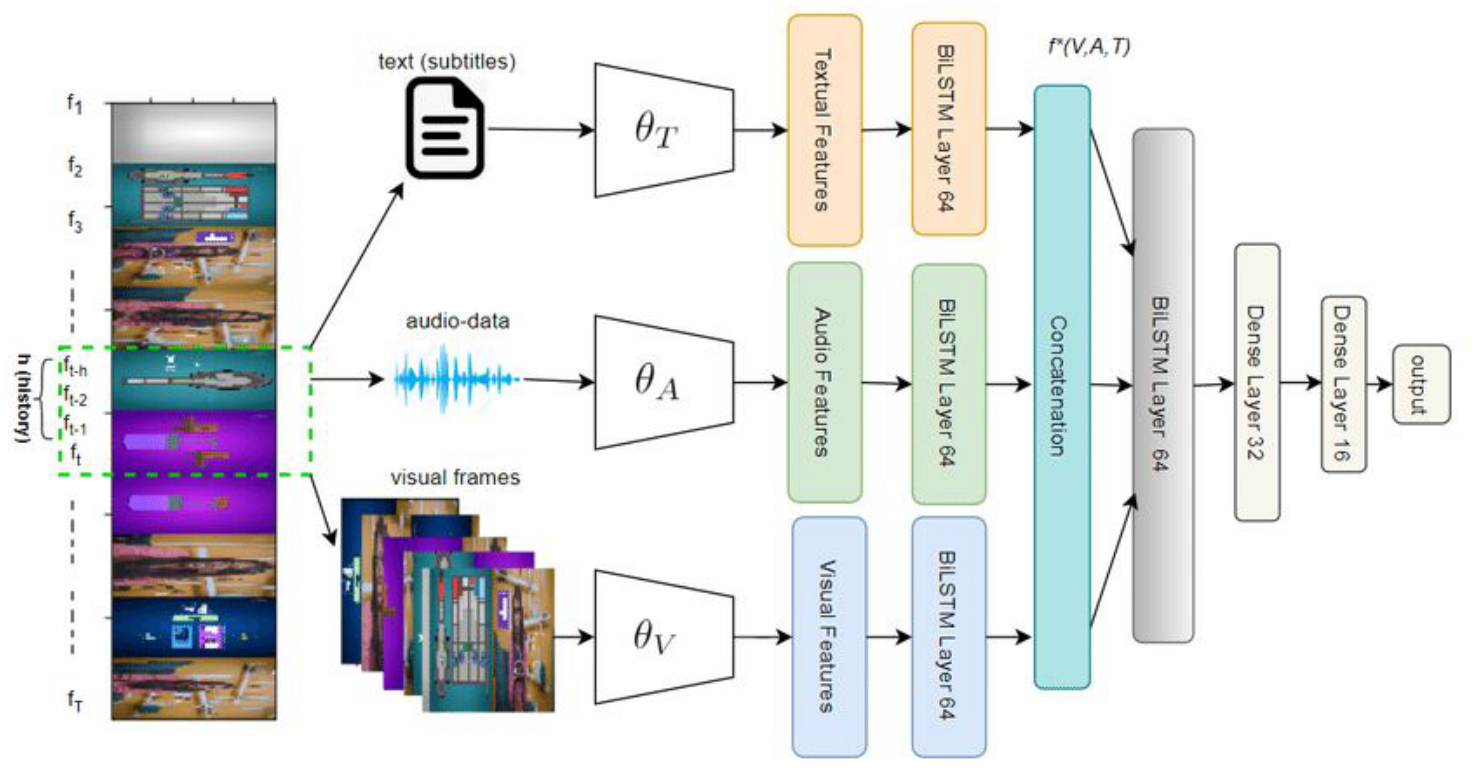
\includegraphics[width=0.85\linewidth, height=0.72\textheight, keepaspectratio]{images/multimodal-nlp-agentic-ai/multimodal_trimodal_text_audio_visual_fusion.png}
        \caption*{\scriptsize Source: Ghauri, Hakimov \& Ewerth, ``Classification of Important Segments in
        Educational Videos using Multimodal Features'', CIKM 2020 Workshops,
        \href{https://arxiv.org/abs/2010.13626}{arXiv:2010.13626}, Figure~2.}
      \end{figure}
    \end{column}
  \end{columns}
\end{frame}

\begin{frame}{Categories of Multimodal Architectures}
  \begin{itemize}
    \item[\textcolor{red}{$\triangleright$}] \textbf{Early Fusion:} Combine the modalities at the input of a
      single shared encoder.\\
      \textit{Example: VisualBERT adds image region embeddings as tokens to the Transformer.}
    \item[\textcolor{red}{$\triangleright$}] \textbf{Late Fusion (dual encoder):} Process each modality
      separately, then merge only at the output.\\
      \textit{Example: CLIP encodes images and text independently, then compares embeddings.}
    \item[\textcolor{red}{$\triangleright$}] \textbf{Hybrid / Cross-modal Attention:} Enable interactions between modalities at multiple stages using attention mechanisms.
  \end{itemize}

  \vspace{0.6em}
  \textbf{Design Considerations:}
  \begin{itemize}
    \item[\textcolor{red}{$\triangleright$}] \textbf{Alignment:} How to align representations across modalities.
    \item[\textcolor{red}{$\triangleright$}] \textbf{Modality Dropout:} Handling missing or noisy modalities during training or inference.
    \item[\textcolor{red}{$\triangleright$}] \textbf{Shared vs. Modality-Specific Layers:} Deciding which layers are shared and which are unique to each modality.
  \end{itemize}
\end{frame}

\begin{frame}{Where Fusion Happens}
  \begin{figure}
    \centering
    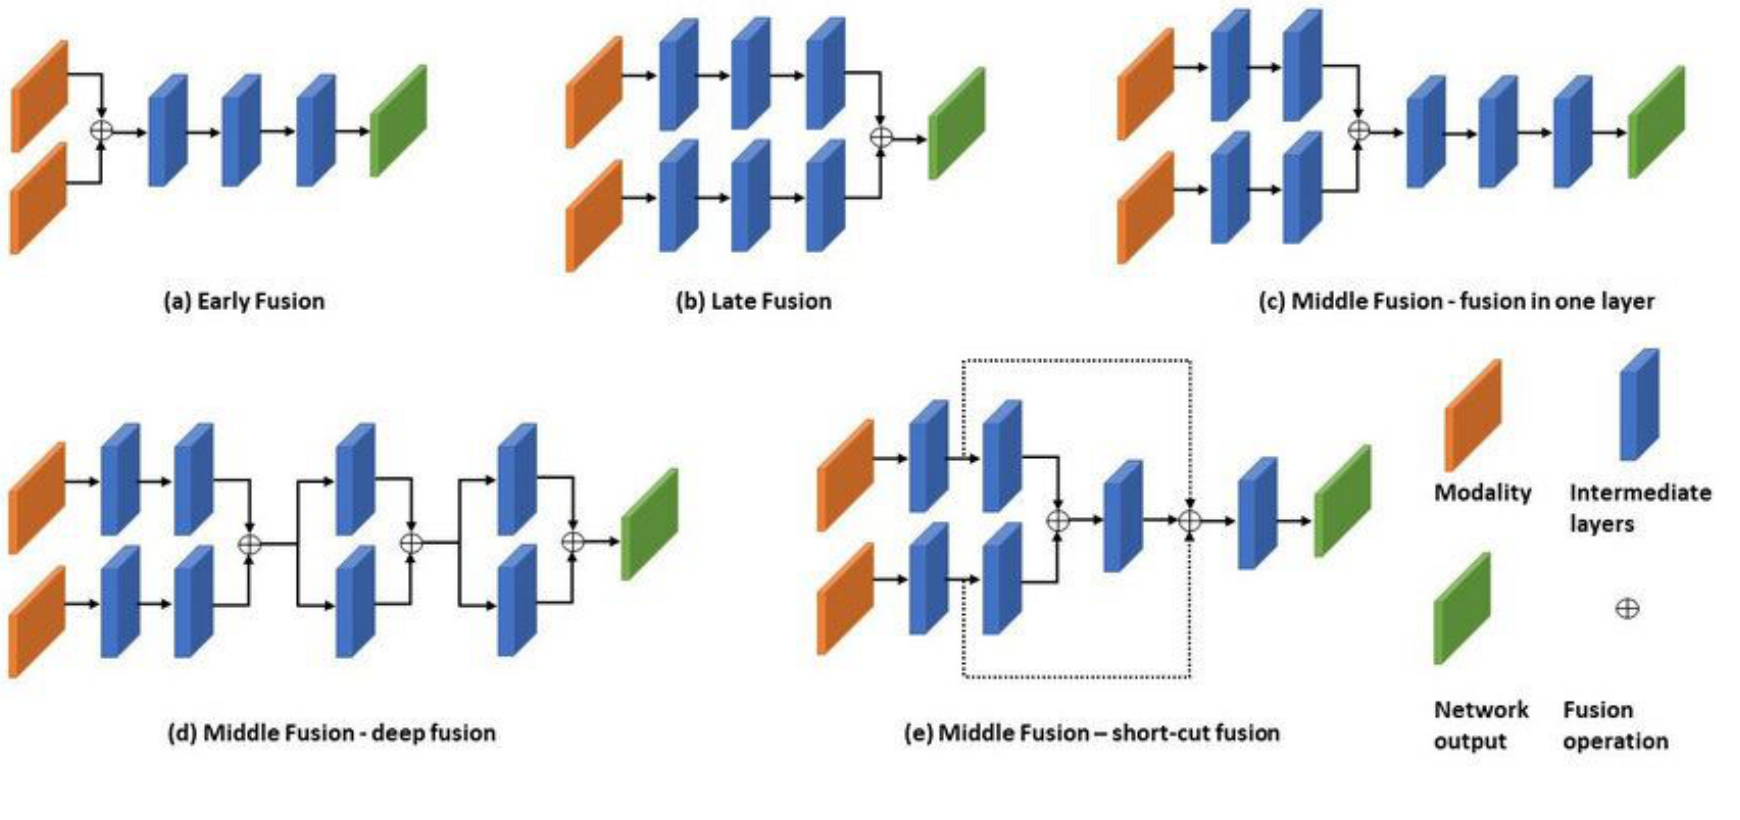
\includegraphics[width=0.98\textwidth, height=0.78\textheight, keepaspectratio]{images/multimodal-nlp-agentic-ai/multimodal_fusion_strategies_diagram.png}
    \caption*{\scriptsize Orange is a modality, blue an intermediate layer, green the network output, and
    $\oplus$ a fusion operation. Middle fusion is the general case: the hybrid, cross-modal-attention
    designs sit here. Source: Feng et al., ``Deep Multi-modal Object Detection and Semantic Segmentation
    for Autonomous Driving'', \href{https://arxiv.org/abs/1902.07830}{arXiv:1902.07830}, Figure~8.}
  \end{figure}
\end{frame}

\begin{frame}{Early Fusion}
  \begin{figure}
    \centering
    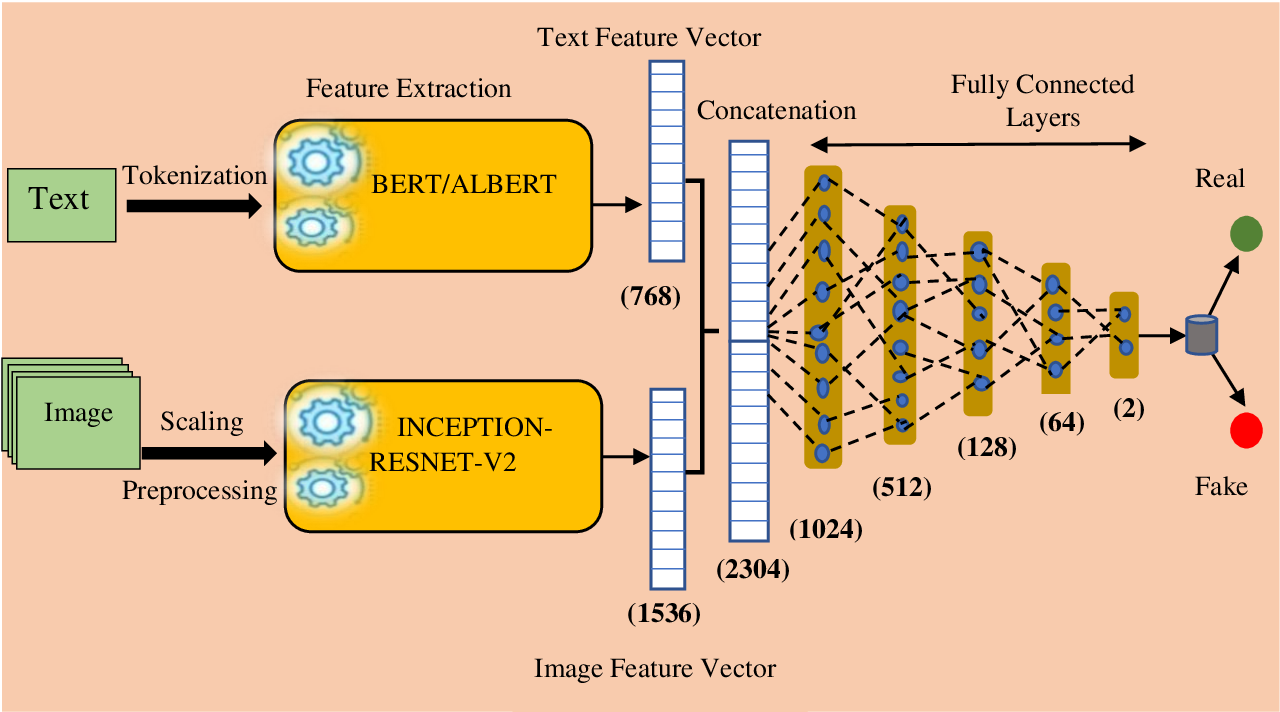
\includegraphics[width=0.98\textwidth, height=0.78\textheight, keepaspectratio]{images/multimodal-nlp-agentic-ai/multimodal_text_image_fakenews_classifier.png}
    \caption*{\scriptsize A fake-news detector: text and image features are concatenated before any
    classification happens, so the dense layers see both modalities at once. Source: Meel \& Vishwakarma,
    \href{https://arxiv.org/abs/2109.12547}{arXiv:2109.12547}, Figure~3.}
  \end{figure}
\end{frame}

\begin{frame}{Late Fusion}
  \begin{figure}
    \centering
    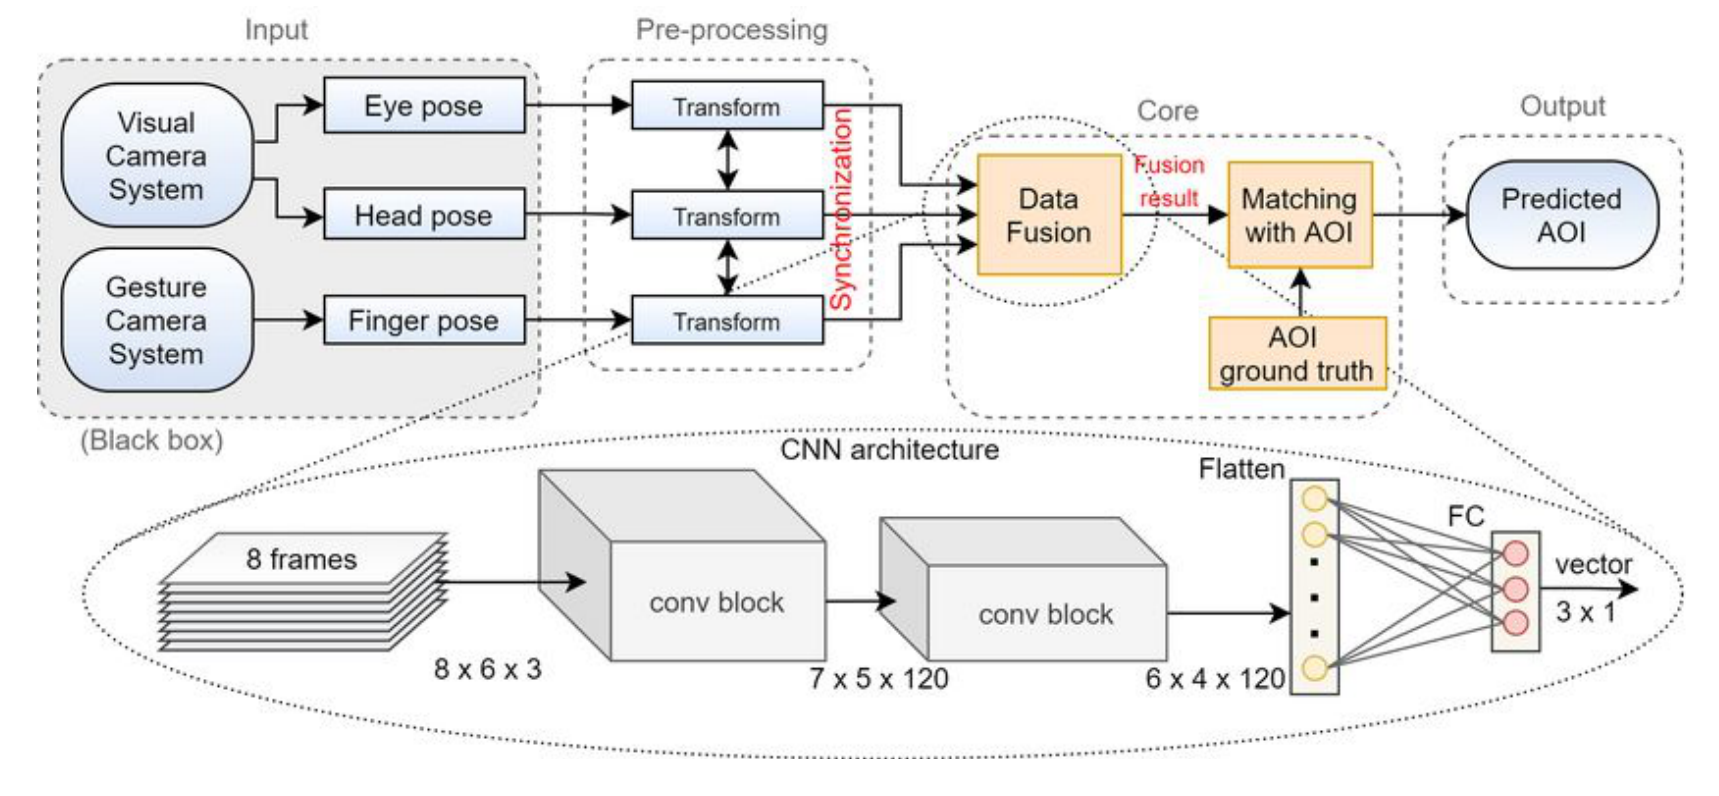
\includegraphics[width=0.98\textwidth, height=0.78\textheight, keepaspectratio]{images/multimodal-nlp-agentic-ai/multimodal_gaze_gesture_data_fusion_cnn.png}
    \caption*{\scriptsize Predicting which object in a car the driver means from gaze, head pose and finger
    pointing: each sensor is processed independently and the streams meet only at the fusion step. Source:
    Aftab, von der Beeck \& Feld, ``You Have a Point There'', \href{https://arxiv.org/abs/2012.13449}{arXiv:2012.13449}, Figure~6.}
  \end{figure}
\end{frame}

\begin{frame}{Challenges in Multimodal Integration}
  \begin{figure}
    \centering
    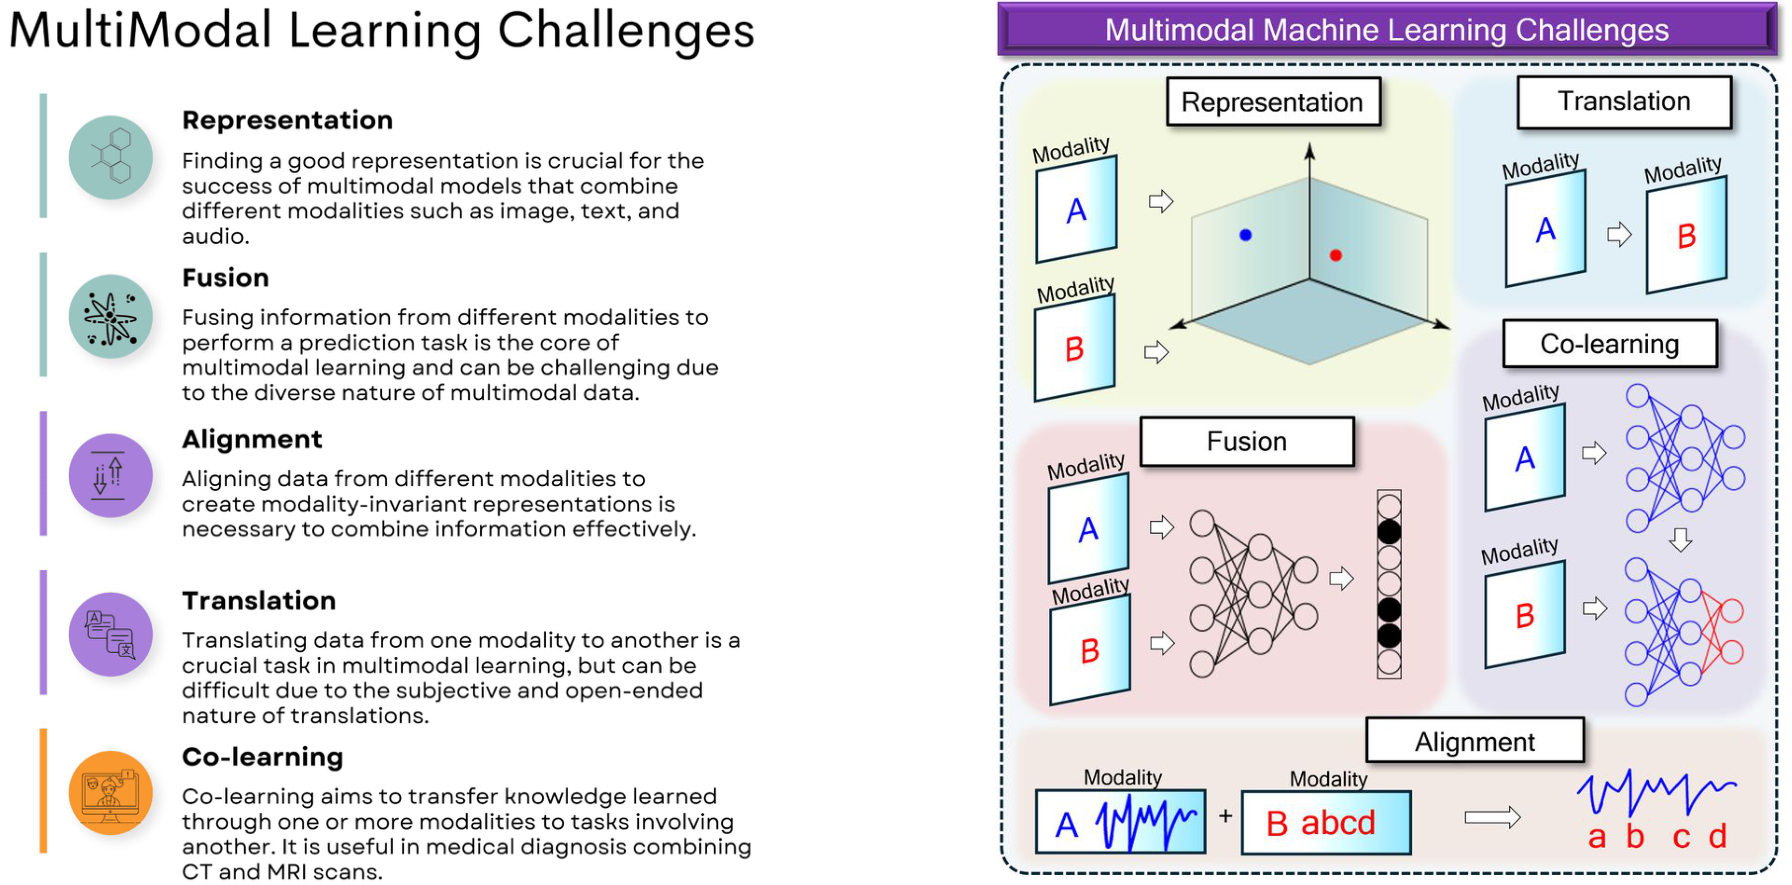
\includegraphics[width=0.98\textwidth, height=0.78\textheight, keepaspectratio]{images/multimodal-nlp-agentic-ai/multimodal_learning_challenges.png}
    \caption*{\scriptsize Representation, fusion, alignment, translation and co-learning: the five-way
    taxonomy of Baltru\v{s}aitis, Ahuja \& Morency, ``Multimodal Machine Learning: A Survey and Taxonomy'',
    \href{https://arxiv.org/abs/1705.09406}{arXiv:1705.09406}.}
  \end{figure}
\end{frame}
